%------------------------------------------------------------------------------------------------------------------------------------------
% Teorie
%------------------------------------------------------------------------------------------------------------------------------------------
\chapter{TEORETICKÁ VÝCHODISKA}
\par Pro plné pochopení, výběru a případné vypracování platformy je potřeba si objasnit a vysvětlit několik témat. V prní řadě to jsou především \textit{Vývojové platformy low-code} -- výsledná platforma by měla splňovat tuto definici. Dále si objasníme pojemy \textit{Business inteligence} -- platforma bude z části pracovat s touto oblasti a \textit{Platforma pro pokročilou vizualizaci dat} -- pro snadné používání uživatelského rozhraní. A vzhledem k tomu že výsledná platforma musí do určité míry pracovat s uživatelskými právy a spravovat uživatele, objasníme si pojem \textit{Server pro řízení přístupu a identity}

\section{Vývojové platformy low-code}
\par Vývojové platformy low-code jsou celkem nový pojem, tyto produkty začaly vznikat, protože malé a střední podniky potřebovaly vytvořit rychle a za použití menšího počtu vývojářů aplikace, které mohou být nadále rychle spravovány. \cite{pcmag-no-coding}

\par Toto v podstatě znamená, že vývojáři mohou rychle měnit software na základě uživatelských požadavků, což má za následek spokojenější uživatele, uživatelsky přívětivější software a to všechno za minimálního použití ručního programování. Tyto platformy neeliminují programování jako takové, ale podporují rychlejší vývoj tak, že poskytují vizuální nástroje a napomáhají konfiguraci datových modulů a díky tomu eliminují problémy spojené s datovou integrací. \cite{low-code-customer-want}

\subsubsection{Výhody low-code platforem}
\begin{itemize}
\item \textbf{Produktivita:} Systémy mohou být vyvíjeny a nasazeny během menšího časového rozmezí, oproti klasickému programování. \cite{low-code-accelerate}
\item \textbf{Reakční schopnost:} Vývojář může často zvolit různé druhy platforem na kterých bude výsledný produkt fungovat -- od mobilních aplikací, až po webové služby. \cite{low-code-accelerate}
\item \textbf{Spolehlivost:} Aplikace mohou být aktualizovány mnohem rychleji, což má za následek jejich stabilitu a spolehlivost. \cite{low-code-accelerate}
\item \textbf{Úspora času a peněz:} Vývojáři mohou vytvořit mnohem více funkcionality za kratší čas, z čehož plyne, že si firma může dovolit menší počet programátorů. \cite{low-code-accelerate}
\item \textbf{Zaměření na samotný vývoj:} Zaměřením se na to co má aplikace dělat, a ne jak to má dělat, se programátoři mohou zaměřovat na funkcionalitu a uživatelskou spokojenost. Při vývoji je také možné cílit více na uživatelské požadavky mnohem rychleji. \cite{low-code-accelerate}
\end{itemize}

\subsection{Příklady low-code platforem}
\paragraph{Microsoft PowerApps}: Vývojová platforma od firmy Microsoft, která dovoluje vytvořit během několika málo kliknutí aplikaci jak pro mobilní platformy, tak jako webové služby. Při spojením této platformy a aplikace Power BI vzniká velice robustní vývojářský nástroj, díky kterému je možné rychle integrovat produkční data do aplikace, kterou budou uživatelé rádi používat. \cite{pcmag-no-coding}
\paragraph{Zoho Creator}: Výhodou této platformy je využití techniky \uv{\tt{drag-and-drop}}, která umožňuje vytvářet aplikace a převážně jejich uživatelské rozhraní bez nutnosti psát jakýkoliv kód. \cite{zoho-review}
\paragraph{Rollbase}: Při používání této platformy vývojář jako první definuje objekty, jejich vlastnosti a vztahy mezi těmito objekty. Po překonání tohoto kroku máme již plně funkční webovou aplikaci, která je použitelná napříč všemi mobilními zařízeními. \cite{what-is-low-code}
\paragraph{Openshift}: Platforma pro vývoj webovým a mobilních aplikací, postavená na kontejnerech, které zajišťují rychlý vývoj a umožňují dedikovat vývojáře na vytvoření jednoduchých funckionalit, které fungují jako samostatné aplikace. \footnote{Takovýmto aplikacím se říká Mikroservise \url{https://smartbear.com/learn/api-design/what-are-microservices/}}, Tyto malé aplikace zaměřující sena jedoduchou funkci se poté za pomocí Openshiftu spojí dohromady a vytvoří jednu velkou platformu. Na Obrázku \ref{openshift-vrstvy} můžeme vidět, z jakých vrstev se skládá Openshift a můžeme pozorovat jednotlivé aplikace znázorněné v nodech, dále můžeme sledovat, jaké nástroje nabízí Openshift vývojářům (management zdrojových kódů -- SCM a kontinuální integrace -- CI/CD).\cite{openshift-overview}
\begin{figure}[h]
\centering
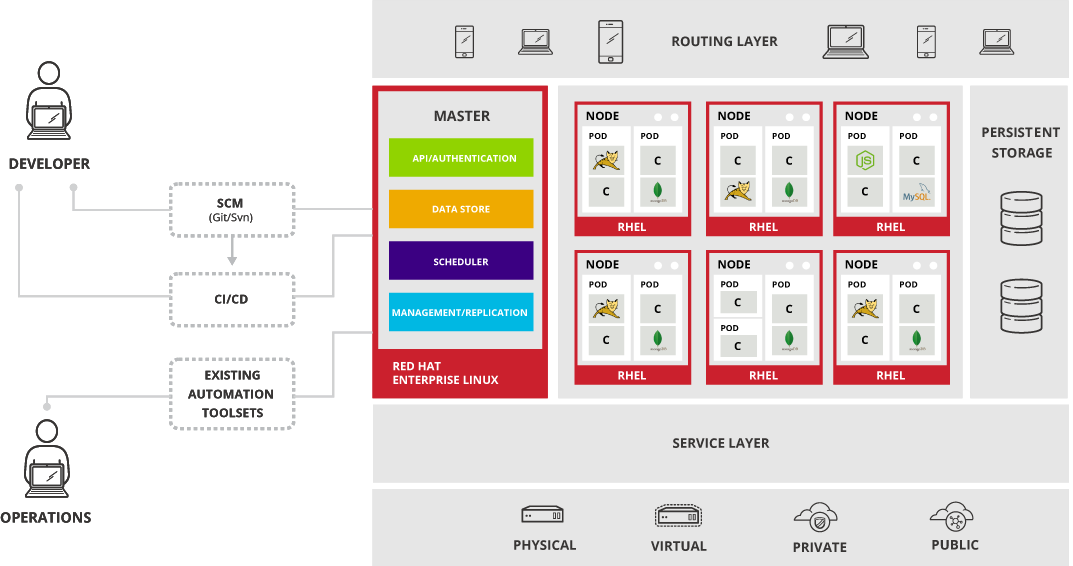
\includegraphics[width=\textwidth]{openshift}
\caption{Znozornění jednotlivých vrstev v platformě openshift.}
\label{openshift-vrstvy}
\end{figure}

\subsection{Cloudový výpočet}
\par Výpočet pomocí cloudu je další fáze ve vývoji internetu, cloud v tomto použití znamená že všechno potřebné pro vývoj a hostování aplikací, až po samostatné stroje je možné nabídnout jako služba kdekoliv na světě se člověk nachází. I když poskytovatelé cloudových řešení mají často velice robustní bezpečnostní systém je na uživateli, který má uložené data v cloudu, aby zajistil jejich bezpečnost. To znamená že pokud data uniknou z cloudu díky špatnému zabezpečení v aplikaci, která je hostovaná, není chyba poskytovatele, ale firmy, která takovou aplikaci vydala.\cite{cloud-computing-dummies}

\par Porovnání ceny cloudového výpočtu a klasického datového uložiště není až tak jednoduché, záleží na několika faktorech. Vezměme si například lokaci datového uložiště, pokud například cena eklektické energie v místě datového uložiště je velice levná firma nemusí být tolik tlačena do cloudového řešení. ale pokud k těmto datům přistupuje velké množství uživatelů z různých koutů světa může se stát že námi poskytované služby budou neresponzivní a uživatelé mohou odejít ke konkurenci. V tomto momentě je potřeba zvážit zda se nám cloudové řešení vyplatí a kdy ne. Důležité je také uvědomit si, že 42 \% nákladů na datové uložiště jde do hardware a software (tyto náklady jsou rozloženy v průběhu času) a 58 \% nákladů jde do topení, klimatizace, daní a samostatné práce. \cite{cloud-computing-dummies}

\subsubsection{Typy cloudového výpočtu}
\begin{itemize}
\item \textbf{Veřejné} dostupné pro širokou veřejnost, jak zdarma, tak placené verze.
\item \textbf{Soukromé} často používané firmami skupinami uživatelů, kteří potřebují zabezpečit data. Často velice drahé a časově nákladné řešení.
\item \textbf{Komunitní} podobné soukromým, ale rozšířené mezi větší skupiny lidí.
\item \textbf{Hybridní} vytvořené z jednoho a více druhů, privátního a nebo veřejného cloudu. Mezi jejich portfolio často patří záloha ke kritickým službám.
\item \textbf{DaaS} data jako služba, pouze data uložené v cloudu.
\item \textbf{PaaS} pro vývoj a hostování celého vývojového cyklu, často včetně možnosti nasazení výsledné aplikace.
\item \textbf{IaaS} infrastruktura jako služba, opravdové, nebo virtuální počítače nabízené uživatelům. \cite{cloud-computing} \label{IaaS}
\end{itemize}

\subsubsection{Platforma jako služba -- PaaS}
Platforma jako služba tento pojem označuje službu, která zahrnuje kompletní škálu nástrojů sloužících pro vývoj aplikací. Od databází, přes aplikační rámce a testovací nástroje až po nasazení a překlad aplikace. Výhoda této služby je převážně v tom, že všechno je přístupné přes internet a často jako webová aplikace, takže není nutné kupovat často velice drahé nástroje. Někteří poskytovatelé nabízí také vyrovnání zatížení, to znamená že pokud je výsledná aplikace pod vysokým náporem uživatelů, automaticky se přiřadí prostředky, aby uživatelé nezaznamenali pád aplikace a bez nutnosti zasáhnout do nastavení služby.\cite{essentials-cloud}

\subsubsection{Výhody PaaS}
\begin{itemize}
\item \textbf{Méně kódu} -- Díky možnosti propojení několika menších aplikací dohromady není potřeba psát stejný kus kódu pořád dokola.
\item \textbf{Nové možnosti bez potřeby nabírání nových lidí} -- Díky PaaS dostane tým do rukou sofistikovanější nástroje.
\item \textbf{Vývoj pro více platform} -- Výhodou mnoha poskytovatelů služby PaaS je možnost překladu aplikací pro různé platformy (několik mobilních platforem a webová aplikace).
\item \textbf{Propojení geograficky nesourodých týmů} -- Pokud je tým rozdělen po různých částech světa služby PaaS dovolují takto rozděleným týmům pracovat efektivněji.
\item \textbf{Efektivní životní cyklus aplikace} -- V rámci integrovaného prostředí se často nachází funkce pro podporu životního cyklu aplikace (sestavení, nasazení, otestování, správa, aktualizace...). \cite{co-je-paas}
\end{itemize}

\section{Bussiness Intelligence}
\par Nástroje pro business Inteligence zahrnují jak samostatná data, tak časovou jednotku, takže můžeme nad těmito daty provádět predikci pomocí sofistikovaných nástrojů a výpočtů. Ze začátku bylo jednoduché provádět takové výpočty, protože jednoduše firma nesbírala takové množství dat. Aktuálně však není v lidských silách provádět takové výpočty nad tak obrovským množstvím dat. \cite{data-science-business}

\par Pravděpodobně nejvíce rozšířeným aplikováním data-miningu je marketing -- sledování nakupování a chování zákazníků. V této oblasti je možné vybrat si každého zákazníka, a v případě že máme dostatek dat, cílit na něj lépe reklamu. \cite{data-science-business}

\par Pro plné využití BI nástrojů potřebujeme sledované subjekty rozdělit do několika skupin, tyto skupiny musí být co nejvíce \textbf{Heterogenní} (rozdílné) vůči sobě, a subjekty v rámci jedné skupiny musí být na druhou stranu co nejvíc \textbf{Homogenní} (stejné). Pokud sledované subjekty spadají do více skupin (toto se může hodit z mnoha důvodů) můžeme použít takzvané \textbf{Clustery}. Což jsou skupiny objektů, které si jsou co nejvíce podobné, ale objekty v jiné skupině se jim budou co nejvíce lišit. \cite{data-science-business} Jak takové clustery vypadají můžeme vidět na obrázku \ref{cluster-fig}, kde jsou tři druhy skupin do kterých jsou jednotlivá data rozdělována.

\begin{figure}[htp]
\centering
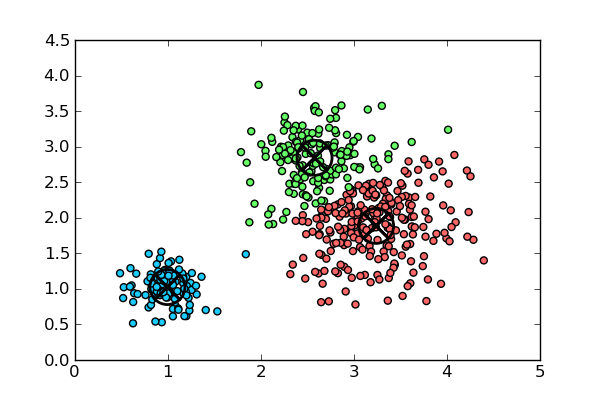
\includegraphics[max size={\textwidth}]{kmeans1}
\caption{Příklad dělení dat do clusterů.}
\label{cluster-fig}
\end{figure}

\par Samostatná data jako taková však nejsou to nejdůležitější, pokud nebudeme schopni vhodně interpretovat a využít data, která jsme nashromáždili jsou nám k ničemu, z toho důvodu vzniklo strojové učení. V podstatě to znamená, že pokud předáme stroji dostatečně velké množství dat a nastavíme správně parametry, tak nám mohou stroje umožnit rychlejší interpretaci takových dat. Ale na předpovědi je nutno nahlížet s odstupem a nebrat je příliš vážně a přesně, naštěstí například pro úspěšný prodej není potřeba přesných předpovědí, stačí pouze vědět kdy a komu poslat přesně cílenou reklamu. Pokud se systém trefí do těchto kritérií je velká pravděpodobnost že si námi zacílený zákazník pořídí produkt, který se mu snažíme prodat. \cite{predictive-analytics}

\subsection{Big data} \label{big-data}
Označení Big data může dostat jakékoliv množství strukturovaných, nestrukturovaných a částečně strukturovaných dat, které mají potenciál k tomu aby z nich bylo možné vydolovat nějaké skryté informace. Ve zkratce to znamená že data začnou výt velkými v momentě, kdy jejich zpracování tradičními metodami je časově a technologicky složité.\cite{big-data-anayitics}

\par Big data lze definovat pomocí pravidla \textbf{3V} -- Volume, Velocity, Variety. Pro přesné definování můžeme vzít v úvahu také Veracity, Validity a Volatility.\cite{big-data-anayitics}
\begin{itemize}
\item \textbf{Volume} -- Ve světě Big data máme na mysli opravdu velké množství dat.
\item \textbf{Velocity} -- Rychlost s jakou jsou data vypracována.
\item \textbf{Variety} -- Různorodostí dat máme na mysli jejich formát (\textit{strukturovaná} -- klasické RDBMS, \textit{částečně strukturovaná} -- emaily, zprávy ...; \textit{nestrukturovaná} -- multimediální obsah).
\item \textit{Veracity} -- Věrohodností rozumíme že data musí být očištěna od zbytečného šumu.
\item \textit{Validity} -- Data musí být co nejpřesnější a co možná nejvhodnější pro naše rozhodování.
\item \textit{Volatility} -- Data musí být co nejaktuálnější pro přesnější predikci a jejich pozdější zpracování. \cite{big-data-anayitics}
\end{itemize}

Nejvhodnější místo pro uložení takového množství dat, je cloud, přesněji využít službu některých poskytovatelů privátních nebo veřejných IaaS. \ref{IaaS} Cloud je vhodný pro Big data převážně kvůli tomu, že jak uložení, tak práce s takovým objemem dat, požaduje velké množství distribuované počítačové síly. \cite{big-data-dummies}

\paragraph{Škálovatelnost} se zaměřením na Hardware znamená že pro Big data je potřeba přejít z relativně malého výpočetního výkonu na velký během několika chvil bez nutnosti změnit architekturu. Pokud budeme mluvit o Softwaru je zapotřebí zachovat stejnou jednotku síly jak se zvětšuje Hardware (při zvýšení objemu dat by mohlo dojít ke značnému poklesu výkonu, pokud na to není systém připraven). \cite{big-data-dummies}

\paragraph{Pružnost} je potřeba zachovat co největší, převážně kvůli tomu že mohou nastat momenty, kdy máme velké množství dat, které se ale v čase mohou smrsknout pouze na zlomek těchto dat. Pokud se tomu tak stane nechceme nadále platit za zbytečně nevyužitý prostor. \cite{big-data-dummies}

\paragraph{Sdružování prostředků} cloud dovoluje vytvářet skupiny sdílených prostředků. \cite{big-data-dummies}

\paragraph{Samoobsluha} většina poskytovatelů cloudových řešení nabízí možnost samostatně, bez nutnosti kontaktovat IT oddělení, navýšit zdroje, případně je odpojit (pokud již nejsou potřebné). Toto je často řešeno nějakým portálem, případně specifickými nástroji u uživatele daného cloudu. \cite{big-data-dummies}

\paragraph{Nízká pořizovací cena} znamená že často cloudové řešení nestojí uživatele tolik jako pořízení drahých datových skladů. \cite{big-data-dummies}

\paragraph{Platba za chodu} se používá u poskytovatelů cloudu jako způsob platby za zdroje, které využíváme. Takže je dost možné že v průběhu používání cloudu budeme platit různé částky. \cite{big-data-dummies}

\paragraph{Tolerance pádů} u cloudových řešení je nutnost a musí být u takovýchto řešení co nejnižší, aby byl zajištěn nepřetržitý chod. \cite{big-data-dummies}

\subsection{Data-mining} \label{data-mining}
\par Pokud budeme potřebovat velkého množství dat (Big data \ref{big-data}), musíme je nejdříve očistit od chybně zapsaných dat. Dokonce i když máme data ve standardní formě nemůžeme počítat s tím, že jsou tyto data naprosto bez chybná. Takto chybně zapsaná data mohou být nicméně důležitá pro náš systém.\cite{data-mining-principles}

\par Dále některé atributy mohou naprosto chybět pro některé záznamy, pro vypořádání s takto chybějícími atributy můžeme zvolit jednu ze dvou taktik. \cite{data-mining-principles}
\begin{enumerate}
\item Odstranění -- jednoduše odstraníme celý záznam ve kterém se nám nachází nějaký chybějící atribut.
\item Náhrada -- použijeme nejvíce frekventovanou, nebo nějakou výchozí hodnotu na místě ve kterém najdeme chybějící atributy. \cite{data-mining-principles}
\end{enumerate}

\par Na obrázku \ref{crisp-dm} vidíme jednotlivé fáze popsané v CRISP-DM \footnote{Zkratka znamená cross-industry process for data mining} modelu, tyto fáze jsou:
\paragraph{Pochopení podniku} na začátek je potřeba pochopit, co za problém se snažíme vyřešit pomocí dolování dat. Tento první krok je nejdůležitější, ze začátku budeme mít pouze slabé pochopení tohoto kroku a v rámci procesu dolování dat se budeme vracet do tohoto bodu. \cite{data-mining-practical}

\paragraph{Pochopení dat} často narazíme na data, která nebudou naprosto sedět zadanému problému, proto se musíme zaměřit na jejich silné a slabé stránky. Často se stává že historická data neodpovídají aktuálním problémům podniku. Další složkou, která se projeví do dat je samozřejmě cena, některé datové sady jsou takřka zadarmo, další se dají pořídit a některá prostě neexistují. Proto v rámci pochopení dat musíme zvážit případné rozšíření datové složky a zda se nám vyplatí investovat do dalších dat. \cite{data-mining-practical}

\paragraph{Příprava dat} je dost možné, že tato část bude předcházet \textbf{pochopení dat}, protože jednoduše pro pochopení dat musíme nejdříve tyto data očistit od případných chybných a chybějících atributů. \cite{data-mining-practical}

\paragraph{Modelování} primární fáze ve které jsou použity techniky pro dolování dat. \cite{data-mining-practical}

\paragraph{Vyhodnocení} po aplikování modelování se nacházíme ve fázi, kde musíme ověřit, zda výsledný model je to co podnik potřebuje. Pokud tomu tak není, vracíme se zpátky na pochopení podniku a opakujeme celé kolečko znovu. Pro vyhodnocování používáme jak kvantitativní tak kvalitativní kritéria. \cite{data-mining-practical}

\paragraph{Nasazení} po vyhodnocení že námi zvolený model je v pořádku a že techniky zvolené pro dolování dat byly korektní aplikujeme výsledek na reálné využití. Bez ohledu na to zda nasazení proběhlo v pořádku vracíme se zpátky do první fáze -- pochopení podniku. Další proces dolování dat může vyvodit jiný model, který může být vhodnější pro daný problém. \cite{data-mining-practical}
\begin{figure}[!htp]
\centering
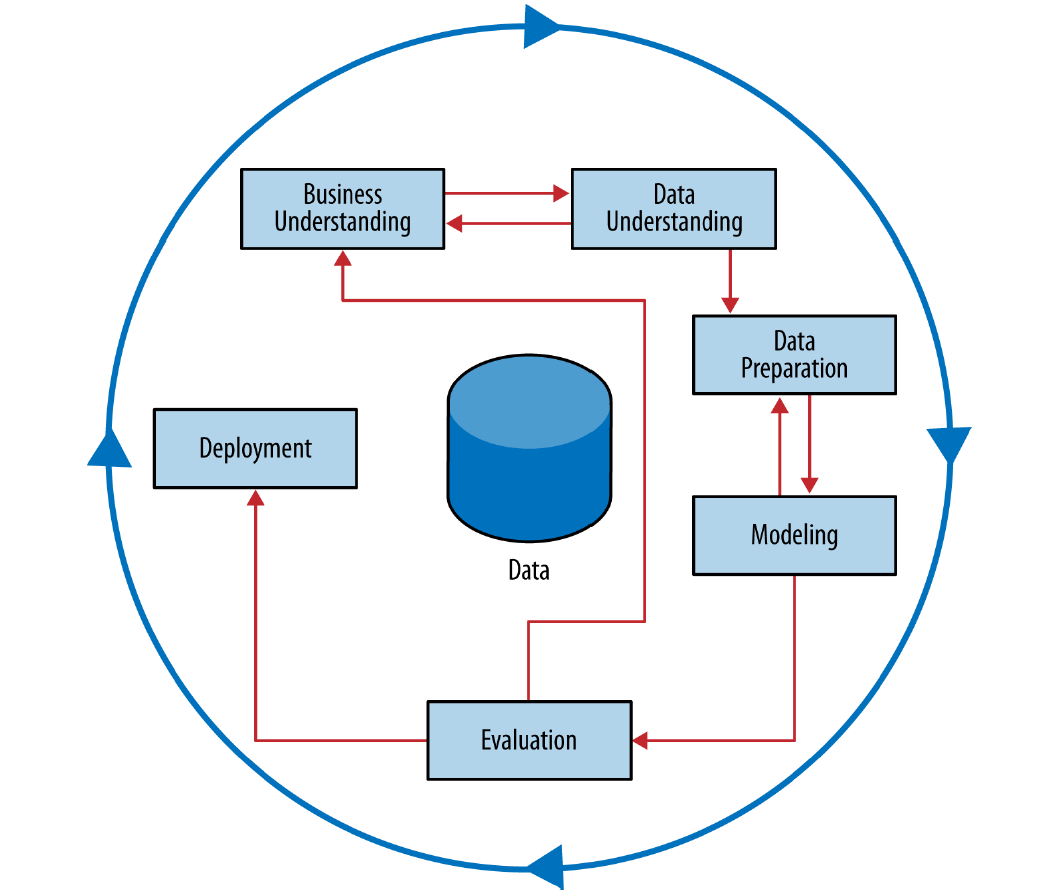
\includegraphics[width=\textwidth]{data-mining-process}
\caption{Fáze CRISP-DM, referenční model.}
\label{crisp-dm}
\end{figure}

\paragraph{Extraction, Transofrmation, Loading}
\par Extraction, Transofrmation, Loading ve zkratce \textbf{ETL} jsou procesy zodpovědné za naplnění dat do datových skladů. Nejdříve jsou data vyextrahována z různých uložišť. Těmito uložišti mohou být OLTP, starší systémy, webové stránky atd. Poté jsou data očištěna, zbavena duplikátů a chybějících atributů. Následně jsou data nahrána do datových skladů, kde se s nimi může dále pracovat.


\section{Platforma pro pokročilou vizualizaci dat}
\par Podniky často zjišťují že vizualizace dat je pro ně důležitým prvkem v odhalování problémů a monitorování podniku. Často se stává že klasické zobrazení dat v podobně reportů za použití tabulek nedokáže zaměřit celý problém, nebo často vede ke špatné analýze. Z toho plyne že je lepší použití grafických prvků jako (jednoduše řečeno grafů), pro ještě lepší usnadnění analýzy je vhodné použít dynamických a interaktivních grafických prvků. Mezi tyto dynamické a interaktivní prvky patří dashboardy, grafy a tabulky které se automaticky aktualizují pokud se jejich datová sada změní.

\subsubsection{Pokročilá vizualizace dat vs. statické grafy}
\begin{itemize}
\item \textbf{Dynamické datové sady} -- Při změně datových sad (databází) se automaticky graf překreslí.
\item \textbf{Vizuální dotazování} --Jednoduchá manipulace s grafy, to znamená například kliknutím na sloupec se provede akce, která má za následek překreslení grafu.
\item \textbf{Několik dimenzí, propojené vizualizace} -- Klasický graf nedokáže zobrazit závislosti mezi několika dimenzemi, proto je vhodné zobrazit provázané grafy, které reagují v závislosti na navigaci v jedné dimenzi. Například -- počet prodaných kusů v čase, při výběru specifického měsíce a roku se automaticky překreslí graf na počet prodaných kusů za den.
\item \textbf{Animované vizualizace} -- Pokud má dimenze velké množství hodnot je vhodné použít animaci pro jednoduché ovládání a znázornění.
\item \textbf{Zosobnění} -- Analytici mohou mít různé pochopení dat a proto je dobré je nechat pracovat individuálně s daty. Často se také může stávat že různí analytici mají přístup k různým datovým sadám, proto je potřeba zajistit pověřovací úrovně.
\item \textbf{Varování pro podnik} -- Pokud se stane že na obrazovce se nachází příliš mnoho dat může se často stávat že analytici jednoduše nebudou schopni odhalit problém včas. Proto by platforma pro pokročilou vizualizaci dat měla nabízet nějaký druh upozorňování. Tato upozorňování však nesmí být pouze grafického typu, ale také ve formě nějaké zprávy v případě že se uživatel nedívá přímo na vizualizaci. \cite{advanced-data-vizualization-platforms}
\end{itemize}

\subsection{Single page aplikace}
\par Tradiční přístup k vývoji webové aplikace je že máme databázi připojenou do serverového back-endu ke kterému jsme schopní se dostat pomocí webového rozhraní. Celá těžká práce je založena na serveru, to znamená navigace, veškerá logika a práva. To často vede k zatížení serveru a má za následek neresponzivní a pomalé aplikace. Z toho důvodu byl vyvinut nový způsob zobrazování aplikace, takzvané \textbf{Single page aplikace} (zkráceně pouze SPA). Tyto aplikace využívají Javascript k vykreslení stránky a navigaci, to znamená méně dotazů na server při přechodu mezi jednotlivými částmi aplikace. V případě že server budeme využívat pouze jako zdroj informací, je možné uživateli doručit intuitivní a snadno použitelnou aplikaci, kdy například ani pád serveru, nefunkční nebo pomalé připojení, nemusí znamenat pád aplikace \footnote{Takovémuto přístupu se říká Service Worker a více se můžete dozvědět na \url{https://developers.google.com/web/fundamentals/getting-started/codelabs/offline/}}. \cite{serverless-singlepage-apps}

\subsubsection{Výhody Single page aplikací}
\begin{itemize}
\item \textbf{Vykreslování} -- Klasické webové aplikace potřebují při většině uživatelských akcí překreslit celou stránku. To vede k pauze, kdy uživatel čeká na zpracování požadavku na serveru a poté vykreslení celé stránky webovým prohlížečem. Pokud je uživatel připojen pomalým připojením, nebo je server zaneprázdněný, může tato pauza vykreslování trvat řádově několik vteřin. V případě použití SPA to není potřeba. Pouze část stránky se vždy překreslí a často není potřeba k takové akci činnosti serveru.
\item \textbf{Responsibilita} -- Takovéto aplikace minimalizují reakční čas tím, že větší část logiky je přenesena k uživateli. Pouze zpracování dat, validaci a autentizaci má na starosti server. Jak jsou tato data zobrazena a případná filtrace je zpracována u uživatele pomocí SPA. Například pokud uživatel filtruje data pomocí výběru sloupce v grafu není potřeba provést získání dat, tím se nezatěžuje server a stránka zůstává nadále responzivní.
\item \textbf{Notifikace} -- Pokud takto napsaná aplikace musí čekat na server může uživateli dát nějakým grafickým prvkem najevo takovou skutečnost. Případně je možné uživatele upozornit na zprávy ze serveru za pomocí \textbf{Webových notifikací}\footnote{Pro detailní popis můžete následovat \url{https://developer.mozilla.org/en-US/docs/Web/API/Notifications_API/Using_the_Notifications_API}.}.
\item \textbf{Přístupnost} -- Díky tomu že jsou SPA napsány jako webové aplikace je možné se k nim dostat odkudkoliv, pokud má uživatel připojení k danému serveru, kde je takováto aplikace uložena.
\item \textbf{Aktualizace} -- V případě aplikací, které jsou uloženy u uživatele je často potřeba vydat aktualizační balíček a uživatel si ho musí nainstalovat. V případě SPA tomu tak není, aktualizace se provádí takřka automaticky stačí na server nahrát novou verzi aplikace. Jediný problém je že si uživatel musí obnovit stránku.
\item \textbf{Multiplatformní} -- Webové aplikace jsou dostupné takřka na všech platformách, od mobilních zařízení až po velkoplošné obrazovky. Limitací je snad pouze používání zastaralých prohlížečů, naštěstí uživatelé začínají používat modernější prohlížeče a chápou nutnost aktualizací. Jak lze vidět na grafu \ref{browser-share}, tak modernější prohlížeč chrome je o hodně používanější než zastaralý prohlížeč Internet Explorer ve verzi 9 a méně. \cite{SPA}
\end{itemize}
\begin{figure}[H]
\centering
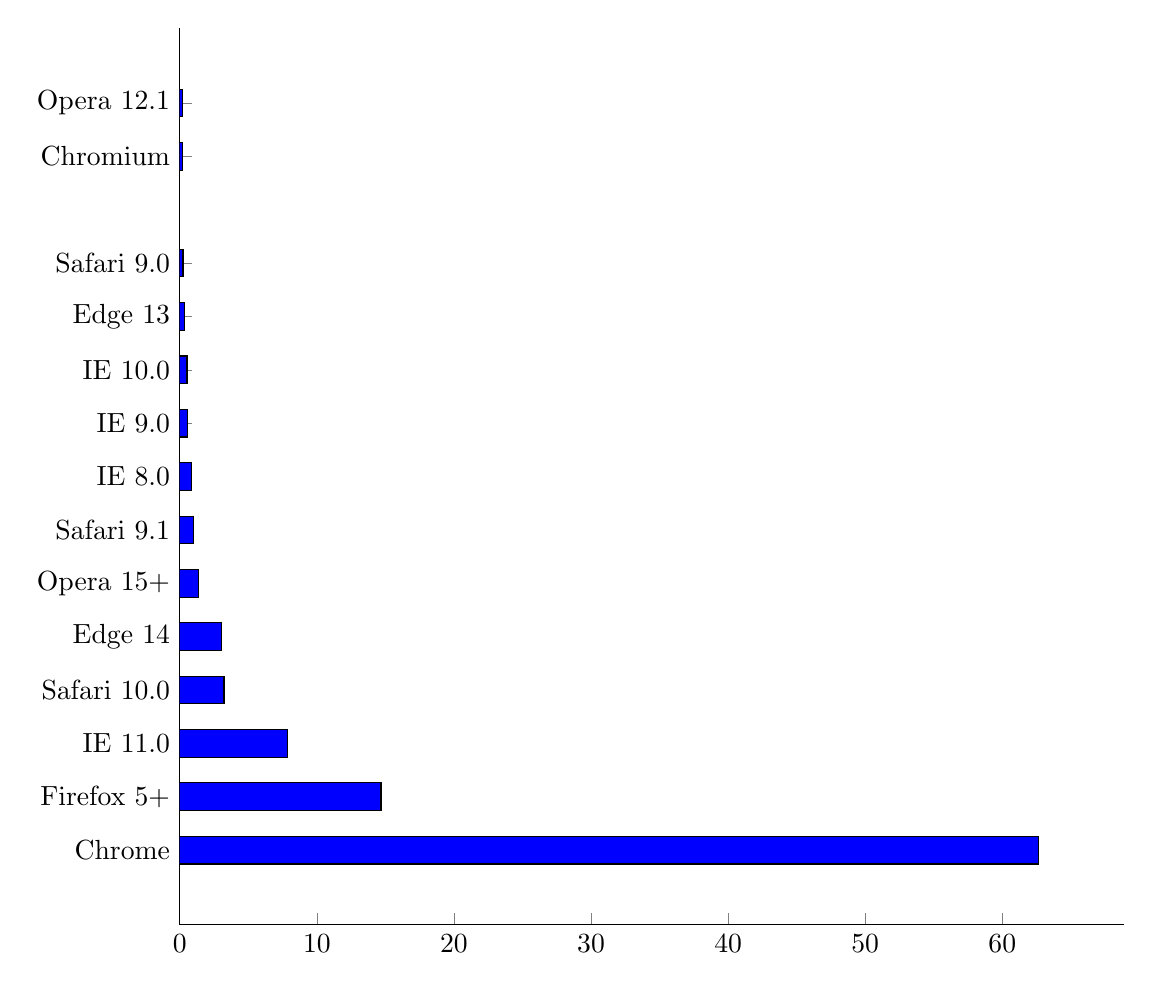
\begin{tikzpicture}
\centering
\begin{axis}[
symbolic y coords={Chrome,Firefox 5+,IE 11.0,Safari 10.0,Edge 14,Opera 15+,Safari 9.1,IE 8.0,IE 9.0,IE 10.0,Edge 13,Safari 9.0,Safari 8.0,Chromium,Opera 12.1,Safari 5.1,Edge 12,Safari 5.0,Safari 6.1,Safari 6.2,Firefox 3.0,IE 6.0,IE 7.0,Other},
ytick=data,
y post scale=2,
x post scale=1.75,
xmin=0,
axis y line*=none,
axis x line*=bottom]
\addplot[xbar,fill=blue] coordinates {
(62.62,Chrome)
(14.68,Firefox 5+)
(7.87,IE 11.0)
(3.23,Safari 10.0)
(3.05,Edge 14)
(1.38,Opera 15+)
(1.01,Safari 9.1)
(0.86,IE 8.0)
(0.54,IE 9.0)
(0.53,IE 10.0)
(0.37,Edge 13)
(0.24,Safari 9.0)
(0.2,Chromium)
(0.18,Opera 12.1)
};
\end{axis}
\end{tikzpicture}
\caption{Podíl vybraných prohlížečů mezi uživateli. Vypracováno na základě dat TODO}
% http://gs.statcounter.com/browser-version-partially-combined-market-share/desktop/worldwide/#monthly-201612-201703-bar
\label{browser-share}
\end{figure}
\subsection{Dynamická a interaktivní vizualizace dat}
\par Problém moderní doby je přehršel informací, proto se lidé snaží najít způsob snadné vizualizace velkého množství dat. Jedním z možných způsobů jak vizualizovat data je pomocí grafů (doslovně je to mapování informací na vizuální objekty), pokud použijeme webových technologií získáme silný nástroj v podobě zatraktivnění takovýchto grafů. \cite{interactive-data-reily}

\par Statická vizualizace je často nepoužitelná a nedostatečná, proto je vhodné použít více grafů najednou, to může vést k nepřehlednosti a ke zmatení. Proto vznikla technologie interaktivní vizualizace, kdy uživatel samotný se snaží vybrat a zpřehlednit data k obrazu svému. interaktivní vizualizace se změnila pouze nepatrně od roku 1996, kdy Ben Shneiderman z Univerzity Marylandu pronesl ,,Nejdříve náhled, poté zoom a filtrování, na závěr detail na vyžádání."\cite{interactive-data-reily}

\par Při vytváření interaktivní vizualizaci dat se musíme zaměřit na 4 fáze návrhu a vývoje. \textbf{Vytvoření designových návrhů} -- kdy navrhneme co a jak bude vypadat v našem systému. \textbf{Realizace alternativ} -- zapracujeme návrhy a vytvoříme první prototypy. \textbf{Verifikace a redefinice návrhů} -- kdy předložíme uživateli námi vytvořené řešení a zapíšeme si jeho reakce a chování. \textbf{Pochopení uživatelských potřeb} -- ze zápisků z předešlého kroku a z požadavků uživatele vyvedeme závěry a opět se vracíme do prvního kroku vytvoření návrhů. Celý koloběh si můžeme prohlédnout na obrázku \ref{data-cycle}. \cite{the-ux-book}

\begin{figure}[h]
\centering
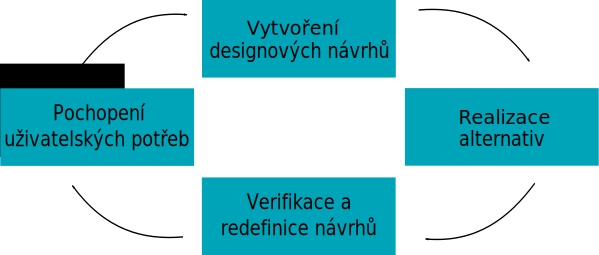
\includegraphics[width=\textwidth]{data_driven}
\caption{Cyklus návrhu grafických prvků.}
\label{data-cycle}
\end{figure}

\subsection{Webová služba RESTful}
\par Od počátku webových služeb server používal takzvané sezení (anglicky \textit{session}), uživateli se při každém načtení stránky přiřadil speciální token, který si server uložil a pracoval s ním pro přístup k datům. Server takto často například ukládal historii navštívených stránek na dané webové stránce, případně filtrovaná data atd. Bohužel ukládání těchto dat vedlo k zahlcení paměti serveru a dlouhým odpovědím ze serveru (kdy server musel často poskládat velké množství dat dohromady). Na základě tohoto se zavedla bez stavová komunikace, kdy si server již nedrží stav o uživatelských akcích, ale odpovídá na všechny dotazy jako na nové sezení. Jedním kdo využívá tohoto bez stavového přístupu k uživatelům je architektický styl RESTful (zkráceně můžeme používat pouze REST). \cite{rest-cookbook}

\subsubsection{Autentizace}
Největším problémem při přístupu k datům, pří použití REST je rozhodně způsob autentizace, server si nedrží přihlášené sezení, ale musí nějakým způsobem odlišit práva jednotlivých uživatelů. Na základě toho vzniklo několik druhů autentizace při použití REST. \cite{rest-cookbook}

\paragraph{Základní přihlášení -- Basic Auth} Uživatel si nejdříve vytvoří učet (nebo je mu přidělen) a na základě toho zná své uživatelské jméno a heslo. Při každém dotazu na server uživatel pošle toto jméno a heslo a server vyhodnotí zda mu pošle data jaká chce. Tento přístup je jednoduchý, ale velice nebezpečný. Jméno a heslo se posílá jako text, který je pouze spojen pomocí \textbf{Base64} do jednoho textu. Pokud server používá nezabezpečené připojení HTTP útočník může toto heslo a jméno jednoduše získat. Při použití zabezpečeného připojení tento problém mizí. \cite{rest-cookbook}

\paragraph{OAuth 1.0} Je zkratka Otevřené autentizace (Open authentication) ve verzi jedna. Při této metodě odpadá problém, kdy uživatel používá více zařízení k přístupu na danou stránku a jedno zařízení by bylo napadeno a uživatel by byl nucen změnit heslo pro všechny zařízení (kde by byl nucen znovu provést přihlášení). Tento problém je řešen tak, že každé zařízení má speciální přihlašovací token a pokud jedno zařízení začne vykazovat špatné chování, uživatel je schopen tomuto zařízení zrušit přístup. \cite{rest-cookbook}

\paragraph{OAuth 2.0} Toto je vylepšený protokol a je momentálně nejvíce rozšířený. Ve zkratce to znamená to, že není nutné pro každé zařízení generovat specifický token, který je možno v případě napadení zařízení zrušit. Tento protokol využívá prostředníka pro uchování klientských údajů. Je to v podstatě to, že služba požádá jiný server, který spravuje daného uživatele o přihlašovací token. Uživatel je přesměrován na adresu třetí serveru, kam zadá své údaje, server poté vyhodnotí správnost těchto údajů a službě která si vyžádala přihlašovací token odešle buď povolí nebo zakáže přihlášení. Výhodou je to, že pokud je uživatel jednou přihlášen na třetím serveru není nutné se znovu přihlašovat. A také pokud uživatel již nevěří službě která má přístup k přihlašovacímu tokenu, jednoduše jí zakáže přístup. \cite{rest-cookbook}

\section{Server pro řízení přístupu a identity}
\par Mnoho firem stále váhá s přechodem z vlastního řešení (jak databázových jednotek, tak aplikací) do cloudu. Hlavní problém je často zabezpečení, firmy jednoduše nechtějí věřit jiné firmě s důvěrnými informacemi, že je ochrání před případným napadením. Naštěstí mnoho poskytovatelů cloudů si toto uvědomuje a tak nemalou část financí investují do robustního autentizačního formátu. \cite{cloud-security}

\subsubsection{Mechanismy používané pro zabezpečení dat v cloudu}
\begin{itemize}
\item \textbf{RSA} -- Pro přihlášení je potřeba HW token, který je synchronizován se servery cloudu.
\item \textbf{Více faktorové} -- Pokud se uživatel chce přihlásit dostane email nebo zprávu s pinem, který po jednom přihlášení, nebo po určitém čase, ztrácí platnost.
\item \textbf{Single sign-on} -- Uživatel je přihlášen ke druhé službě a ta jej autorizuje vůči aplikaci, kterou se chystá použít. Výhoda je ta, že není nutnost vždy zadávat přihlašovací údaje, při přístupu k aplikaci je vyžádán od druhé služby takzvaný JSON web token. \cite{cloud-security}
\end{itemize}

\subsection{JSON Web Token}
\par Zkráceně JWT jsou standard pro autentizaci napříč aplikacemi. Takový token nezávisí na programovacím jazyce, nese veškeré informace (přihlašovací údaje a svůj podpis) a je jednoduše použitelný (může být součástí hlavičky nebo součástí dotazu). \cite{scotch-jwt}

\par JWT je text, který je zakódování pomocí base64 a rozdělen do 3 částí:

\paragraph{Hlavička} obsahuje typ a hashovací algoritmus použitý pro dekódování podpisu.

\paragraph{Náklad} zde se nachází data, která služba poskytuje. Často jsou zde přihlašovací údaje (uživatelské jméno a čas vypršení), dále může obsahovat jakákoliv data chceme, například pohlaví uživatele, věk, email, atd.

\paragraph{Podpis} je text, který vznikne spojením hlavičky a nákladu, který je poté zahashován pomocí algoritmu, který je určen v hlavičce tokenu. Součástí tohoto algoritmu také může být tajné heslo. \cite{rfc-jwt}

\par Příklad jak vypadá zakódovaný a odkódovaný token můžeme vidět na \ref{jwt-token-fig}, kde obsah dat, která JWT nese jsou jméno uživatel, zda je administrátor a čas tokenu. Jak lze vidět, tak součástí hlavičky je také algoritmus použitý pro zakódování.

\begin{figure}[htp]
\centering
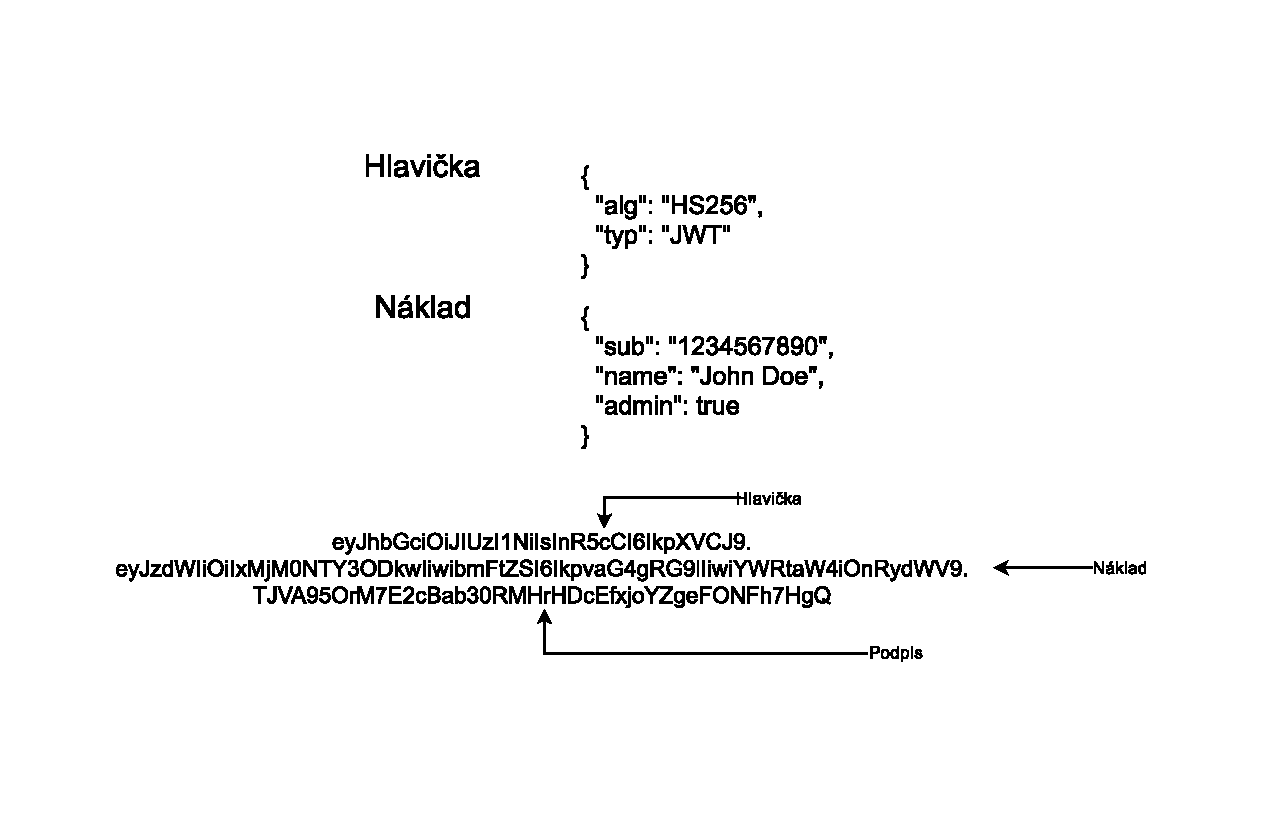
\includegraphics[max size={\textwidth}]{jwt-token.pdf}
\caption{Příklad zakódovaného a odkódovaného JWT.}
\label{jwt-token-fig}
\end{figure}
